\section{Methodology}

It is expected that even in highly entropic or variable packet data, there will be some level of standardization (i.e. method names or status codes) or some commonalities such as user names, device details, semantic contexts, and other conversation or implementation-specific indicators. In order to delve deeper into these hidden layers and capture more latent space representations in packets, we propose in \textsc{Maple} to transform packets into grayscale images, hypothesizing that packets will appear similar to one another once transformed into their image representations. We base this assumption on previous work~\cite{lim2019network} which has shown similarities in grayscale images rendered from packet data in order to classify traffic by application and protocol type which are detectable by CNNs. Figure~\ref{fig:grayscale} asserts the validity of this assumption by showing comparative images rendered from packets in our combined dataset previously used and explained in detail in chapter 4 of this work.

\begin{figure} [ht!]
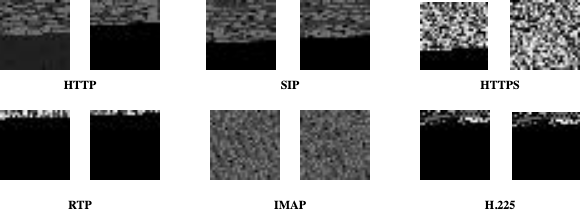
\includegraphics[width=\linewidth]{chapters/5/img/grayscaleimages.drawio.png}
\caption{Grayscale images generated from packets in our combined dataset used in the following experiments.}
\label{fig:grayscale}
\end{figure}

To shape packet payloads into an image, we extract the payloads and convert them from byte encoding to a normalized decimal integer $i \in [0,255]$~\cite{jo2020packet}. For image size, we chose a $28\times28$ representation, for a total of 784 input features. In cases where the payload is shorter than 784 bytes, we apply padding for input normalization, or otherwise truncate the payload data.

\subsection{LeNet Model Configuration}

\begin{figure} [ht!]
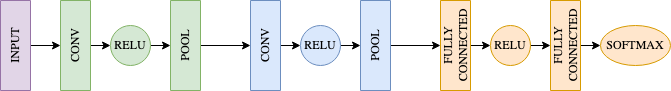
\includegraphics[width=\linewidth]{chapters/5/img/lenet.drawio.png}
\caption{The architecture of our LeNet models.}
\label{fig:lenet}
\end{figure}

We selected LeNet as a standard model in order to test the efficacy of convolutional neural networks to the RTP detection problem. LeNet has a low complexity, so has higher potential for practical use in real-time, line-rate packet inspection systems than deeper models which require more time. Figure~\ref{fig:lenet} shows the set up of the model which we use as a baseline. We designed two separate models where one employed $6$ and $16$ kernels per convolutional layer (A) and another that used a $16$ and $32$ kernels (B). Each model contained two fully-connected, dense layers of size $1024$ with a binary softmax classifier at the output layer.

\subsection{ResNet Model Configuration}

\begin{figure} [ht!]
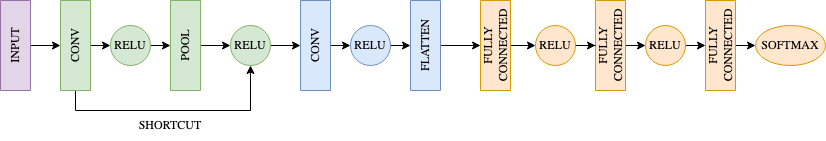
\includegraphics[width=\linewidth]{chapters/5/img/resnet.drawio.png}
\caption{The architecture of our ResNet models.}
\label{fig:resnet}
\end{figure}

For deployment purposes in real network environments, it is imperative that artificial intelligence solutions are capable of scaling to line-rate while still being able to perform the classification task to the required level of accuracy. While the definition of line-rate varies per network environment, the identity mappings of ResNet do not introduce additional complexity~\cite{resnet}. Thus, we introduce residual mapping as a potential solution to adding additional layers of representation and thus improve classification through more hidden features, while also minimizing overhead.

We developed four ResNet-based models for the \textsc{Maple} system's experiments. The first model (C) consists of three convolutional layers with $32$, $32$, and $64$ kernels of dimension $3\times3$, and three dense layers with output sizes of $64$, $32$, and $2$ respectively. The second model (D) follows a similar architecture except the values are halved. Convolutional layers had $16$, $16$, and $32$ kernels per layer and the three dense layers had output sizes of $32$, $16$, and $2$. Model (E) corresponds to the same number of kernels and output sizes as (C), except it uses a kernel dimension of $7\times7$. For all models, the adam optimizer was used as well as ReLU activation between all layers except the final, which used softmax for normalization and classification. Categorical cross-entropy was used as the loss function for training. We also employed a dropout layer in order to reduce model overfitting.

\begin{table} [h!]
\centering
\begin{tabular}{| l | l | l | l | l |}
\hline
Type & Model & \# Kernels & Kernel Size & FC Dim \\
\hline
LeNet & A & $3\times3$ & 6, 16 & 1024, 2 \\
\cline{2-5}
& B & $3\times3$ & 16, 32 & 1024, 2 \\
\hline
ResNet & C & $3\times3$ & 32, 32, 64 & 64, 32, 2 \\
\cline{2-5}
& D & $3\times3$ & 16, 16, 32 & 32, 16, 2 \\
\cline{2-5}
& E & $7\times7$ & 32, 32, 64 & 64, 32, 2 \\
\cline{2-5}
\hline
\end{tabular}
\caption{Configurations of each model used in the experiments.}
\label{table:attacks}
\end{table}
